\documentclass[unknownkeysallowed,12pt,mathserif]{beamer}
\usetheme[secheader]{pecostalk}
\usepackage{graphicx}
\graphicspath{{figs/}}     
\setbeamertemplate{caption}{\raggedright\insertcaption\par}

\setlength{\floatsep}{5pt plus 1.0pt minus 2.0pt}

\date{December 10, 2015}
\author[C. G. Cameron]{Christopher G. Cameron}
\institute{The University of Texas at Austin}
\title[CSE 380 Project]{CSE 380 Project}
\subtitle{Finite Element Solution of the Heat Equation}

\begin{document}
\begin{frame}
\begin{center}
\end{center}
\titlepage
\begin{flushright}
\end{flushright}
\end{frame}

%===============================================================================
% Introduction: Goals for the Project
%===============================================================================
\begin{frame}
\frametitle{Project motivation and goals \ldots}

\begin{itemize}
\item My work is almost exclusively experimental in nature, giving me freedom in project choice
\item Goals
\begin{itemize}
\item Write a significant amount of code from scratch
\item Use a large array of tools from the coursework
\item Object oriented implementation
\end{itemize}
\end{itemize}

\begin{figure}[!htbp] 
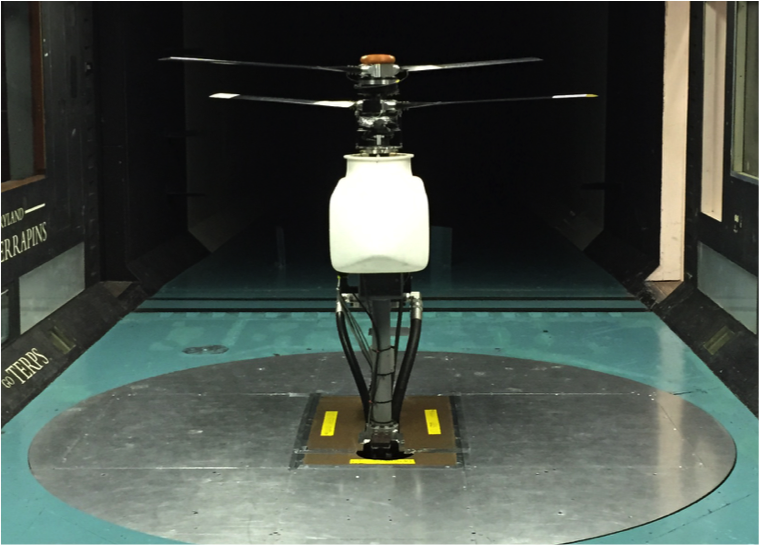
\includegraphics[height = 3cm]{rotor_test_stand.png}
\end{figure}

\end{frame}

%===============================================================================
% Introduction: The Finite Element Method
%===============================================================================
\begin{frame}
\frametitle{Finite Element Method \ldots}

\begin{itemize}
\item The finite element method involves solving a variational form of a differential equation
\item Test and trial functions are chosen as a summation of function with finite support making all integrations local
\end{itemize}

\begin{equation}
   \footnotesize -\frac{d}{dx}\left(k(x)\frac{du}{dx}\right) = f(x) \longrightarrow \sum_{i = 1}^n\sum_{j = 1}^n \int_a^b k(x)\frac{du_i}{dx}\frac{dv_j}{dx}\,dx. = \sum_{i = 1}^n\int_a^b f(x)u_i\,dx.
\end{equation} 

\begin{figure}[!htbp] 
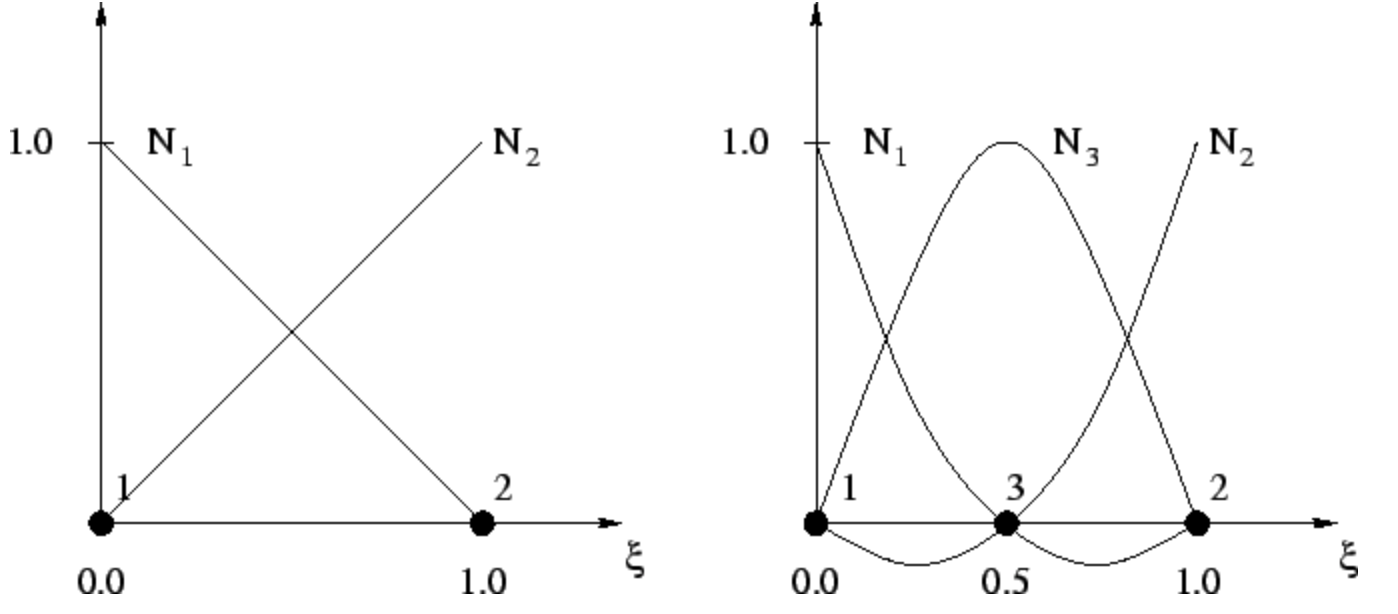
\includegraphics[height = 3cm]{shapes.png}
\end{figure}
\footnotetext{\tiny Mustafa Radi, 1998}

\end{frame}


%===============================================================================
% Introduction: The Finite Element Method
%===============================================================================
\begin{frame}
\frametitle{My code \ldots}

\begin{itemize}
\item Solves the 1D steady heat equation with 1st and 2nd order finite elements, using GRVY for input parsing and timing
\item Objects include: 
\begin{itemize}
\item Domain containing vectors of elements, edges, and nodes
\begin{itemize}
\item Elements point to member nodes and edges, have method for calculating stiffness and forcing matrix contributions
\item Edges point to member nodes and have routine for adding nodes for higher order approximations
\item Nodes know their position and global number
\end{itemize}
\item Solver to hold stiffness matrix and forcing and perform iterative solving
\begin{itemize}
\item Hand coded jacobi and Gauss-Seidel iterative solvers
\item Built in eigen Conjugate Gradient solver
\item Includes output option for comparison with MASA exact solution
\end{itemize}
\end{itemize}
\end{itemize}

\end{frame}

%===============================================================================
% Make System and Version Control
%===============================================================================
\begin{frame}                                                                                                                                                                          
\frametitle{Source control and Make System}
\begin{center}

\begin{figure}[!htbp] 
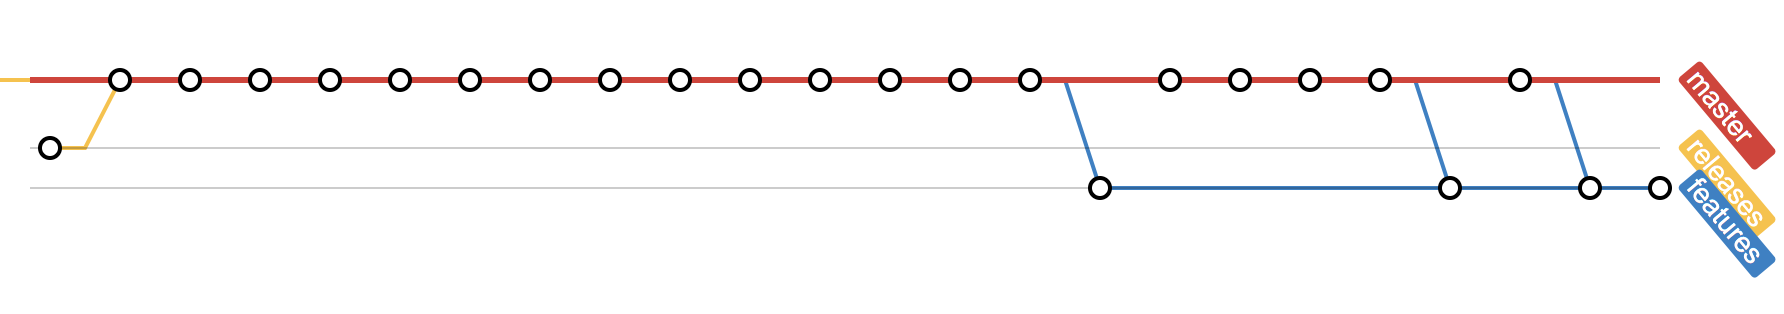
\includegraphics[width=.8\linewidth]{git_graph.png}
\caption{\footnotesize Project commit tree\footnotemark}\label{fig:ct_fit}
\end{figure}

\begin{itemize}

\item Code written in C++

\begin{itemize}
\item External libraries: MASA, GRVY, Eigen
\end{itemize}

\item Makefile based build system with subfolders for sources, external includes, build files, and binaries
\item Git repository on github for version control

\begin{itemize}
\item Most work done on the master branch
\item Branch for GRVY features due to compilation issues on local machine
\end{itemize}

\end{itemize}

\end{center}

\footnotetext{\tiny Git vizualization by gitflowchart}
\end{frame}   

%===============================================================================
% NEW SLIDE
%===============================================================================
\begin{frame}                                                                                                                                                                          
\frametitle{Verification framework}
\begin{columns}[c]
\begin{column}{6.5cm}
\begin{block}{}
\begin{itemize}
\item {Catch unit testing library}
\begin{itemize}
\item Header only
\item Simple asserts with macros
\item Spread tests across multiple files
\item Sections for reusing setup objects
\end{itemize}
\item MASA manufactured solution library
\begin{itemize}
\item 1d Steady heat equation solution for verification
\item Wrapper object created for forcing evaluation due to late integration into code
\end{itemize}
\end{itemize}
\end{block}
\end{column}

\begin{column}{5cm}
\includegraphics[scale=0.21]{catch.png}
\end{column}
\end{columns}

\end{frame}

%===============================================================================
% MASA Verification
%===============================================================================
\begin{frame}

\frametitle{MASA Verification}

\begin{columns}[c]
\begin{column}{6.5cm}
\begin{figure}[!htbp] 
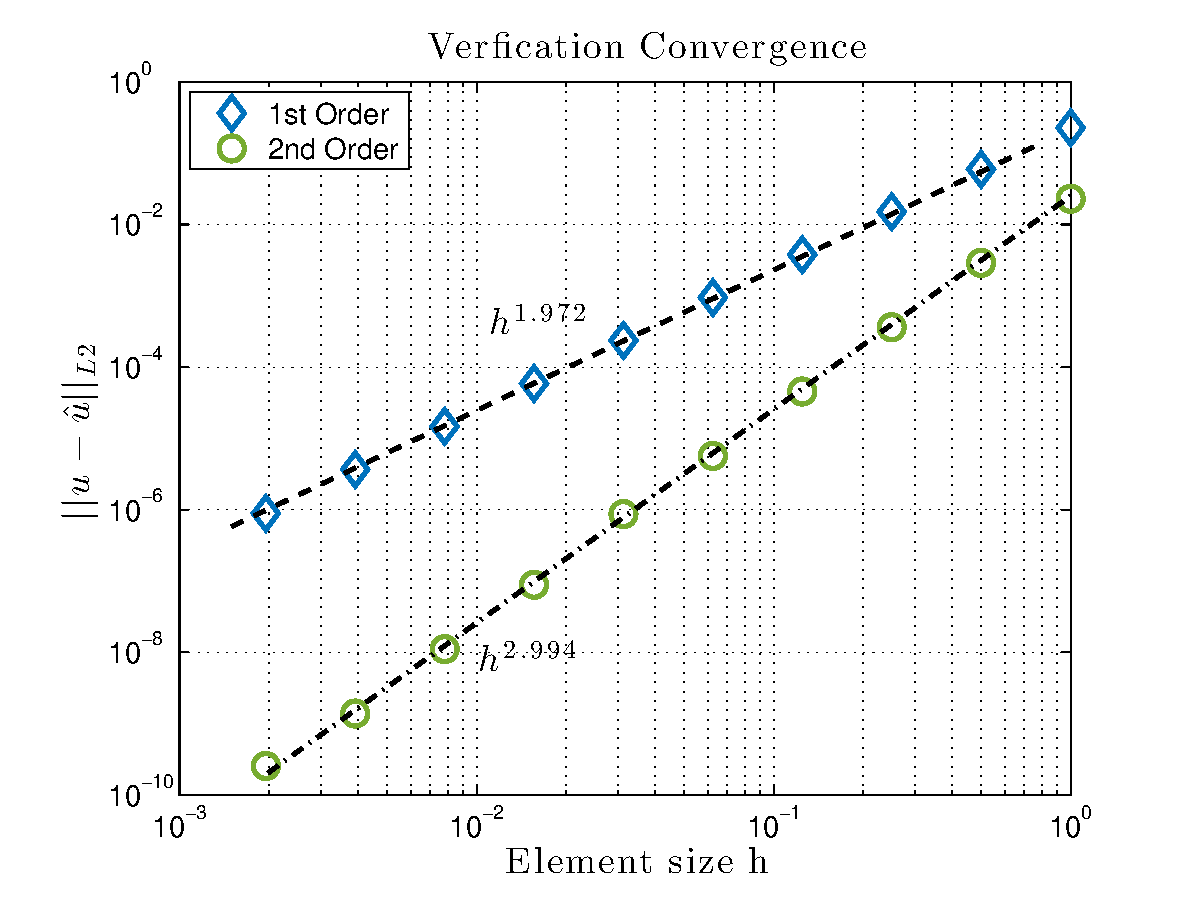
\includegraphics[width=6.5cm]{convergence.eps}
\end{figure}
\end{column}
\begin{column}{6.5cm}
\begin{figure}[!htbp] 
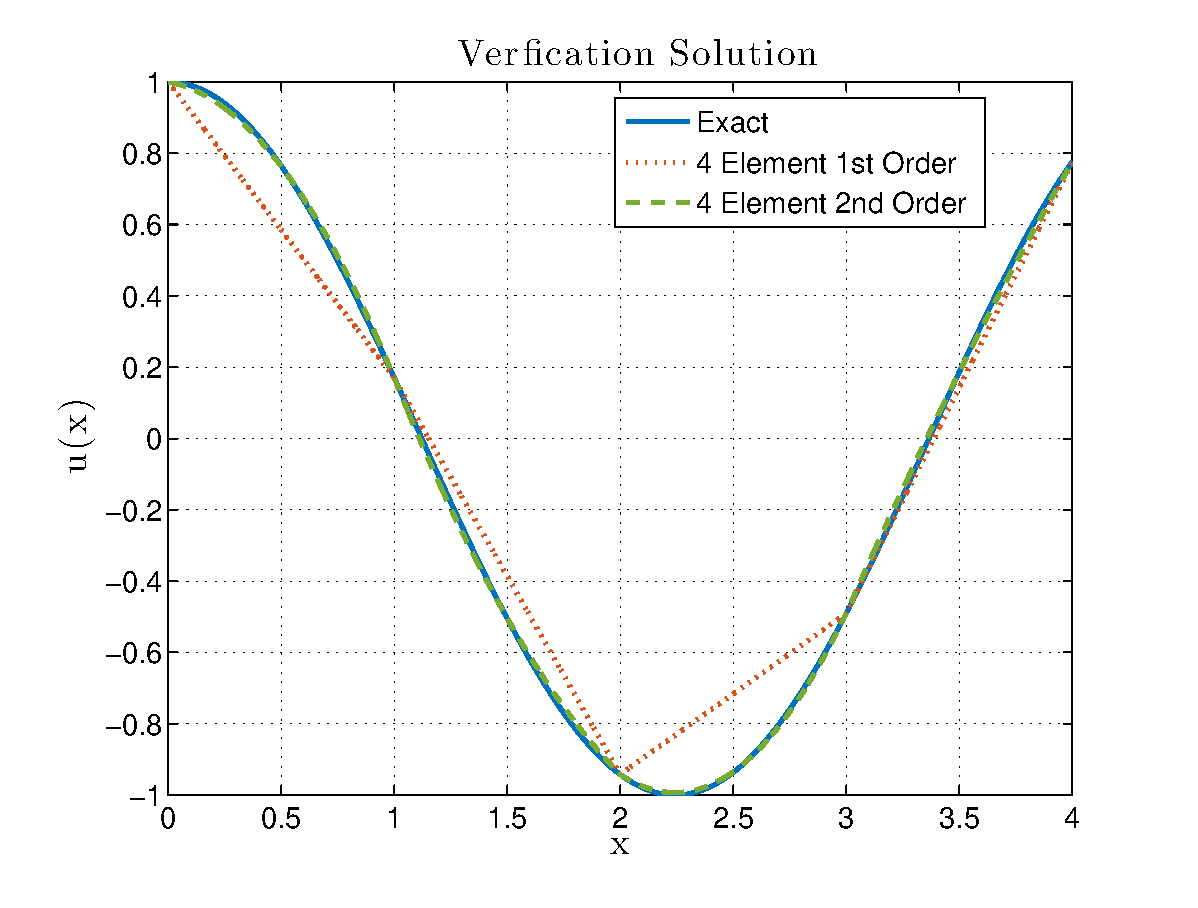
\includegraphics[width=6.5cm]{interpolation.eps}
\end{figure}
\end{column}
\end{columns}
\begin{itemize}
\item \small Convergence of 1st and second order elements is approximately order 2 and 3 respectively, in agreement with theory
\item \small Higher order elements can provide significant gains in accuracy for sufficiently smooth problems
\end{itemize}

\end{frame}

%===============================================================================
% Timing and performance
%===============================================================================
\begin{frame}

\frametitle{Timing and Performance}

\begin{columns}[c]
\begin{column}{6.5cm}
\begin{figure}[!htbp] 
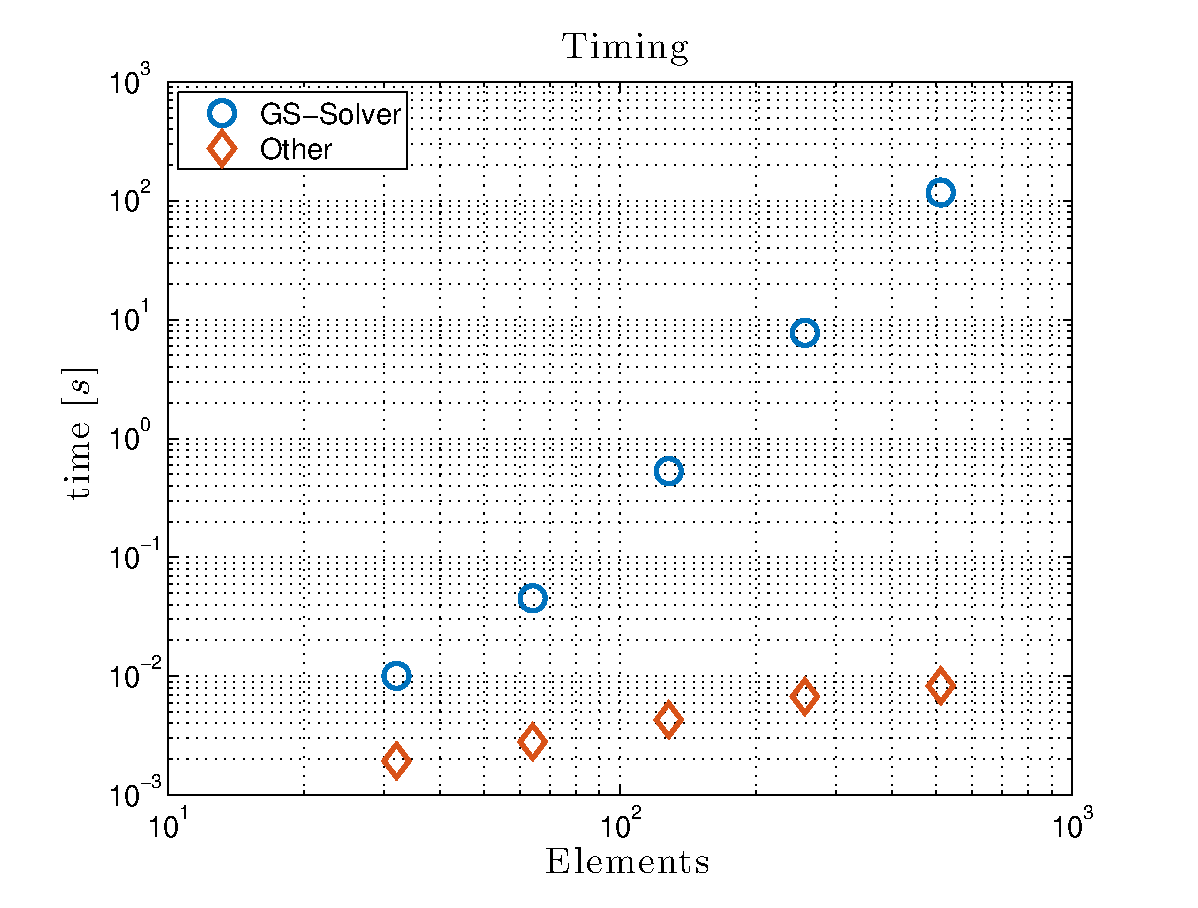
\includegraphics[width=6.5cm]{timing.eps}
\end{figure}
\end{column}
\begin{column}{6.5cm}
\begin{figure}[!htbp] 
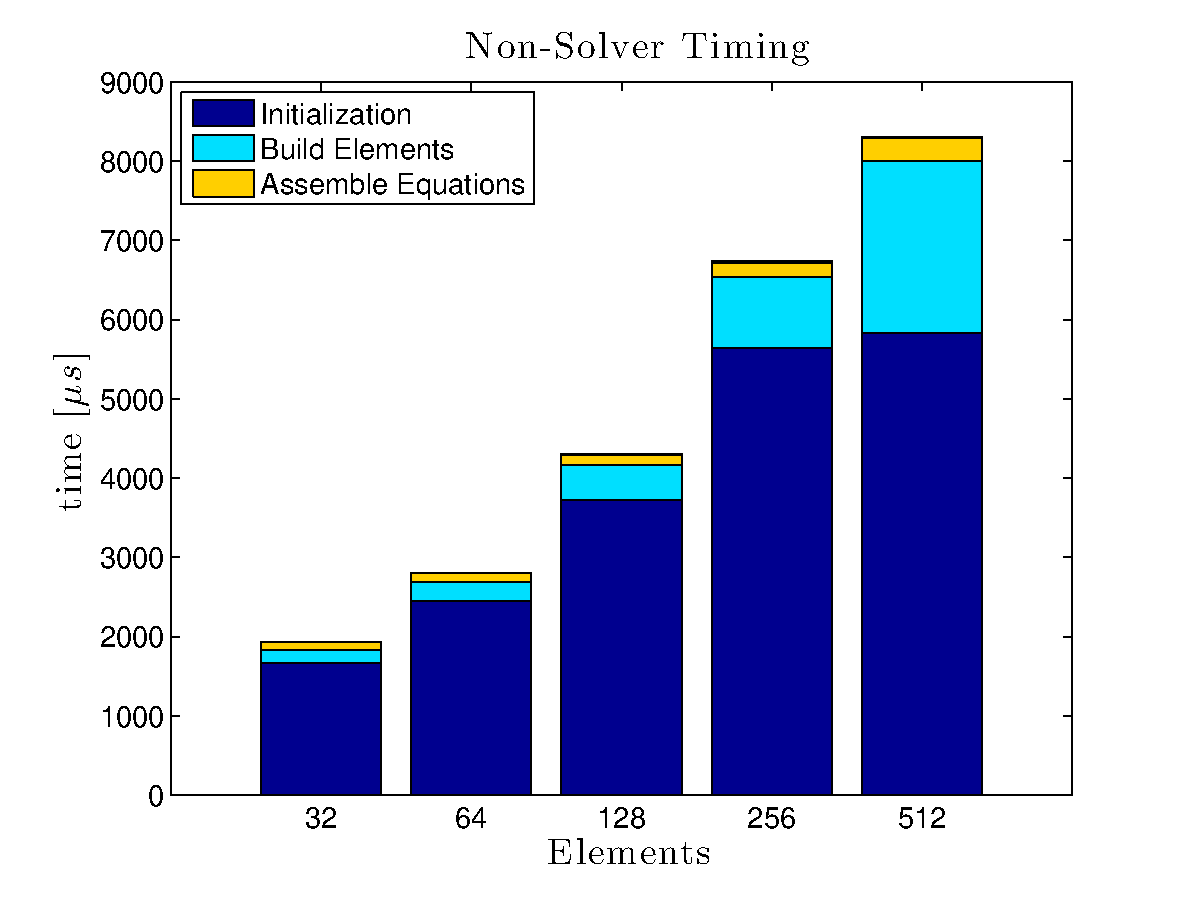
\includegraphics[width=6.5cm]{other_timing.eps}
\end{figure}
\end{column}
\end{columns}
\begin{itemize}
\item \small Program runtime is dominated by the solver routines
\item \small Initialization (parsing input, reserving memory, initializing masa) takes the majority of the rest of the program time
\item \small Meshing and creating nodes, edges and elements takes more time than performing the integrations 
\end{itemize}

\end{frame}
%===============================================================================
% Timing (Continued)
%===============================================================================
\begin{frame}

\frametitle{Timing and Performance}

\begin{columns}[c]
\begin{column}{6.5cm}
\begin{figure}[!htbp] 
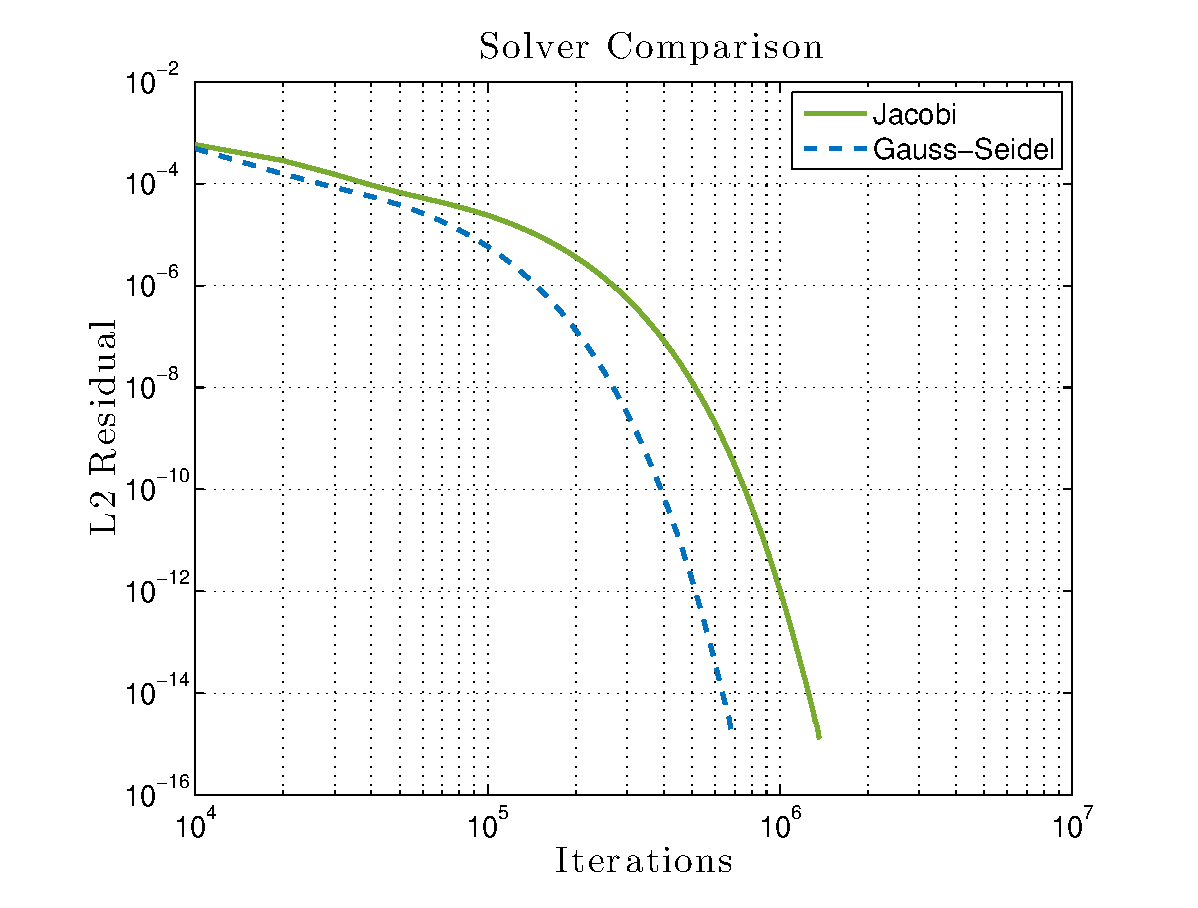
\includegraphics[width=5cm]{solver_convergence.eps}
\end{figure}
\end{column}
\begin{column}{6.5cm}
\begin{figure}[!htbp] 
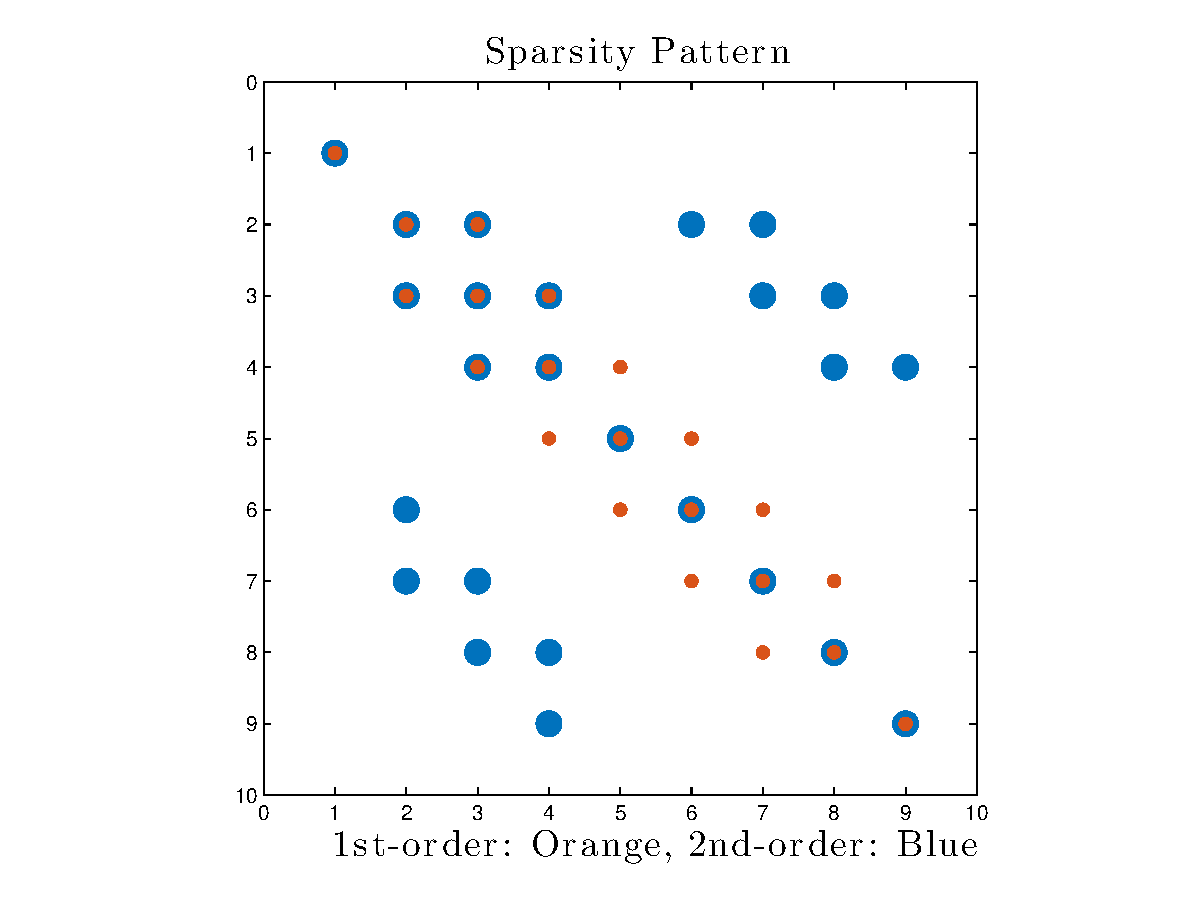
\includegraphics[width=6.5cm]{sparsity.eps}
\end{figure}
\end{column}
\end{columns}
\begin{itemize}
\item \small Gauss-Seidel converges in fewer iterations than the jacobi solver
\item \small The jacobi solver does not converge for 2nd order finite elements
\item \small Using an eigen built-in Conjugate Gradient solver saw ~3000x speedup (vs. GS, n = 256, 2nd order)
\end{itemize}

\end{frame}

%===============================================================================
% Project Flow: How it all went down
%===============================================================================
\begin{frame}
\frametitle{Conclusions \ldots}

\begin{itemize}
\item Began by taking a basic program structure for the 2D problem and implementing in matlab (1 afternoon)
\item C++ coding began with getting unit testing framework setup
\item Tests written at the same time as objects
\begin{itemize}
\item Very useful (except when you write your tests wrong)
\end{itemize}
\item Despite having a solid structure in place before beginning, coding went much slower than expected
\item Late integration of MASA caused some headaches with evaluating forcing and boundary conditions
\item Code is very close to being able to convert to 2d, however the work to make this flexible limited my chances to do more in depth profiling/optimization
\end{itemize}

\end{frame}


%===============================================================================
% NEW SLIDE
%===============================================================================
\begin{frame}
\frametitle{}
\begin{block}{}
\center{Thank you!} \\
\center{Questions?}
\end{block}
\end{frame}

 
\end{document}

\end{document}
